%!TEX spellcheck
%!TEX root = ../bachelor_paper.tex
\documentclass[../bachelor_paper.tex]{subfiles}
\graphicspath{{\subfix{images/}}}
\begin{document}

\chapter{Results}
    \label{ch:res}
    
We were able to successfully generate performance profiles for the benchmarking workloads described in Section \ref{sec:bench/sum}. The workloads vary highly in instruction distribution, however for most of them, arithmetic instructions are the dominant instruction type overall (see Figure \ref{fig:res/overall/inst}). Not all workloads tested support hardware loops. Of those which do, most of them display vastly different \ac{HWL} utilization, depending on the algorithm implemented. We will talk more about this in the following. Of special note is almost 75\% of workloads take more than 50\% of branches (see Figure \ref{fig:res/overall/branch_tk}). Given the \emph{branch not taken} approach taken in RI5CY, this incurs high branching penalties. However, it also indicates a loop-heavy algorithm. In fact, all five programs with a load coefficient less than 1 (meaning less instructions loaded from level 2 than executed) have a branch taken percentage well above 50\% (we intentionally excluded \texttt{tak} included in the \emph{custom} set here, as it only executes 2555 instructions is thus too small to draw conclusions from). 

The opposite conclusion is not possible however, as loop size also matters with regards to the harsh constraint of a 4 instruction preload buffer. \texttt{nettle aes} and \texttt{nettle sha256} have a branch taken rate of 53.68\% and 91.22\% as well as a fetch coefficient of 0.91 and 0.71 respectively. Meanwhile Dhrystone only managed a fetch coefficient of 1.39 with a branch taken rate of 64.89\%. 

This also ties in the above mentioned \ac{HWL} utilization. There is no obvious correlation visible between average \ac{HWL} distance, branch taken rate, and fetch coefficient.

There not being any or little correlation between those metrics is in fact a good thing. The less correlation there is between these data points, the less chance for bias exists when adding a similarity profiler on top of these data sets. In future works we will explore the possibilities for benchmark selection given a certain real life workload and a set of possible benchmark applications.

Lastly, we have identified three major types of programs given their temporal behavior. Not all benchmarks have been analyzed in regards to temporal behavior changes given the relatively short length of some of them. The graphs of those which have been analyzed can be found in Appendix \ref{ch:graphs}. Group 1 does not majorly change its behavior over the duration of the benchmark. All metrics are unchanged over the entire run. One example for group 1 is Dhrystone as seen in Figure \ref{fig:res/dhrystone/inst} and Figure \ref{fig:res/dhrystone/fetch_waste}. The \ac{HWL} graph for Dhrystone is missing, as Dhrystone does not utilize \acp{HWL}. Group 2 shows sectional behavior changes, where sections have relatively stable behavior with stark changes between sections. An example for group 2 would be \texttt{bitcount}, the temporal behavior graphs of which can be seen in Figure \ref{fig:res/bitcount/inst}, Figure \ref{fig:res/bitcount/hwl}, and Figure \ref{fig:res/bitcount/fetch_waste}. Group 3 fluctuates strongly during the entire duration of the benchmark. Examples for group 3 are the synthetic Coremark, as can be seen in Figure \ref{fig:res/coremark/inst}, Figure \ref{fig:res/coremark/hwl}, and Figure \ref{fig:res/coremark/fetch_waste}, as well as \texttt{sglib-combined}, as seen in Figure \ref{fig:res/sglib/inst}, Figure \ref{fig:res/sglib/hwl}, and \ref{fig:res/sglib/fetch_waste}.

%% Overall
\begin{figure}
    \centering
    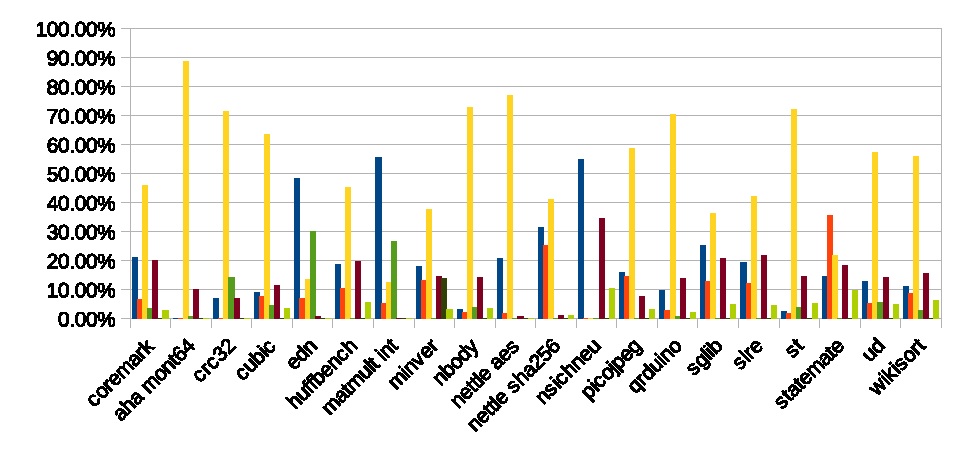
\includegraphics[width=\textwidth]{graph/overall_inst_dist}
    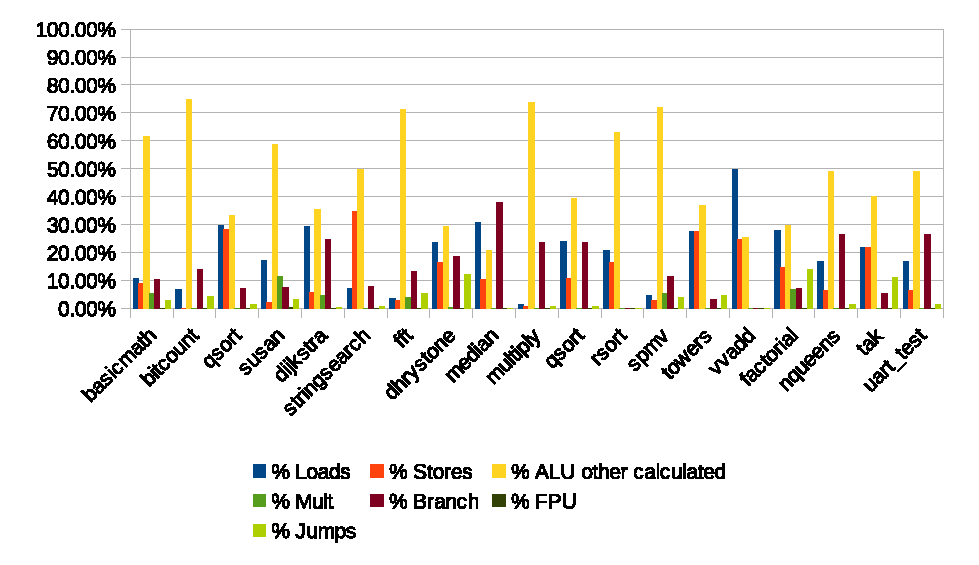
\includegraphics[width=\textwidth]{graph/overall_inst_dist2}
    \caption{Overall instruction distribution of all tested benchmarking workloads}
    \label{fig:res/overall/inst}
\end{figure}

\begin{figure}
    \centering
    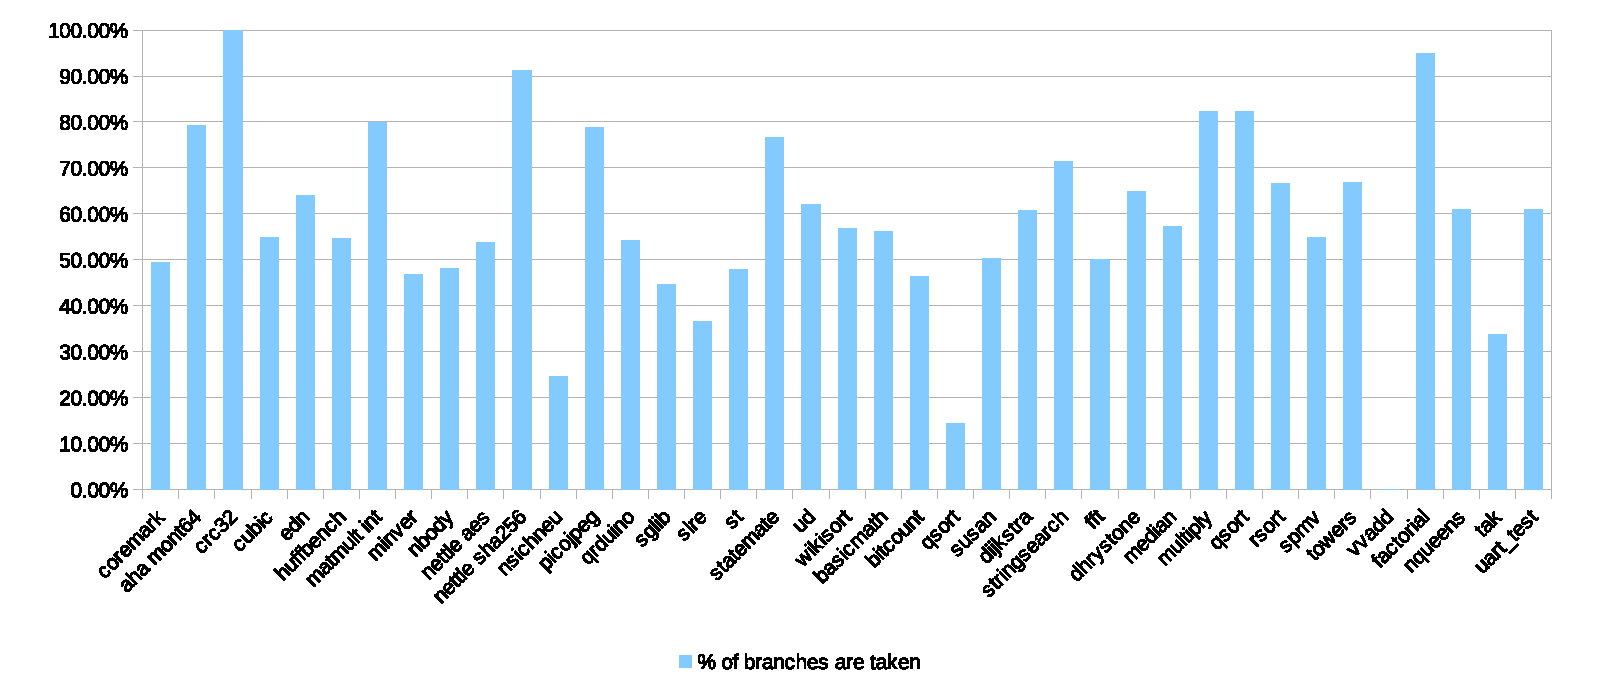
\includegraphics[width=\textwidth]{img/graph/overall_branch_tk.eps}
    \caption{Overall branch taken behavior of all tested benchmarking workloads}
    \label{fig:res/overall/branch_tk}
\end{figure}

\begin{figure}
    \centering
    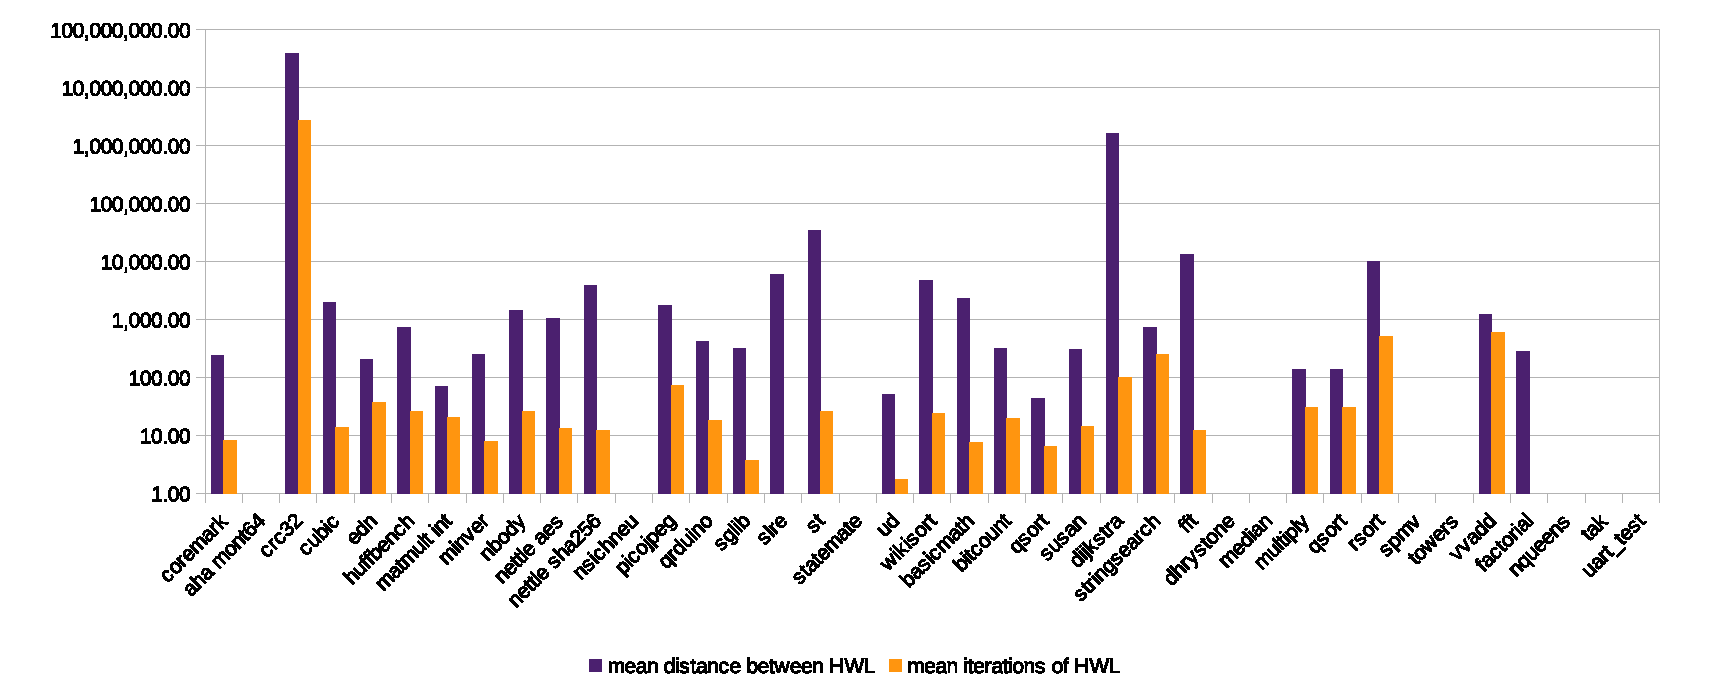
\includegraphics[width=\textwidth]{img/graph/overall_hwl.eps}
    \caption{Overall hardware loop behavior of all tested benchmarking workloads}
    \label{fig:res/overall/hwl}
\end{figure}

\begin{figure}
    \centering
    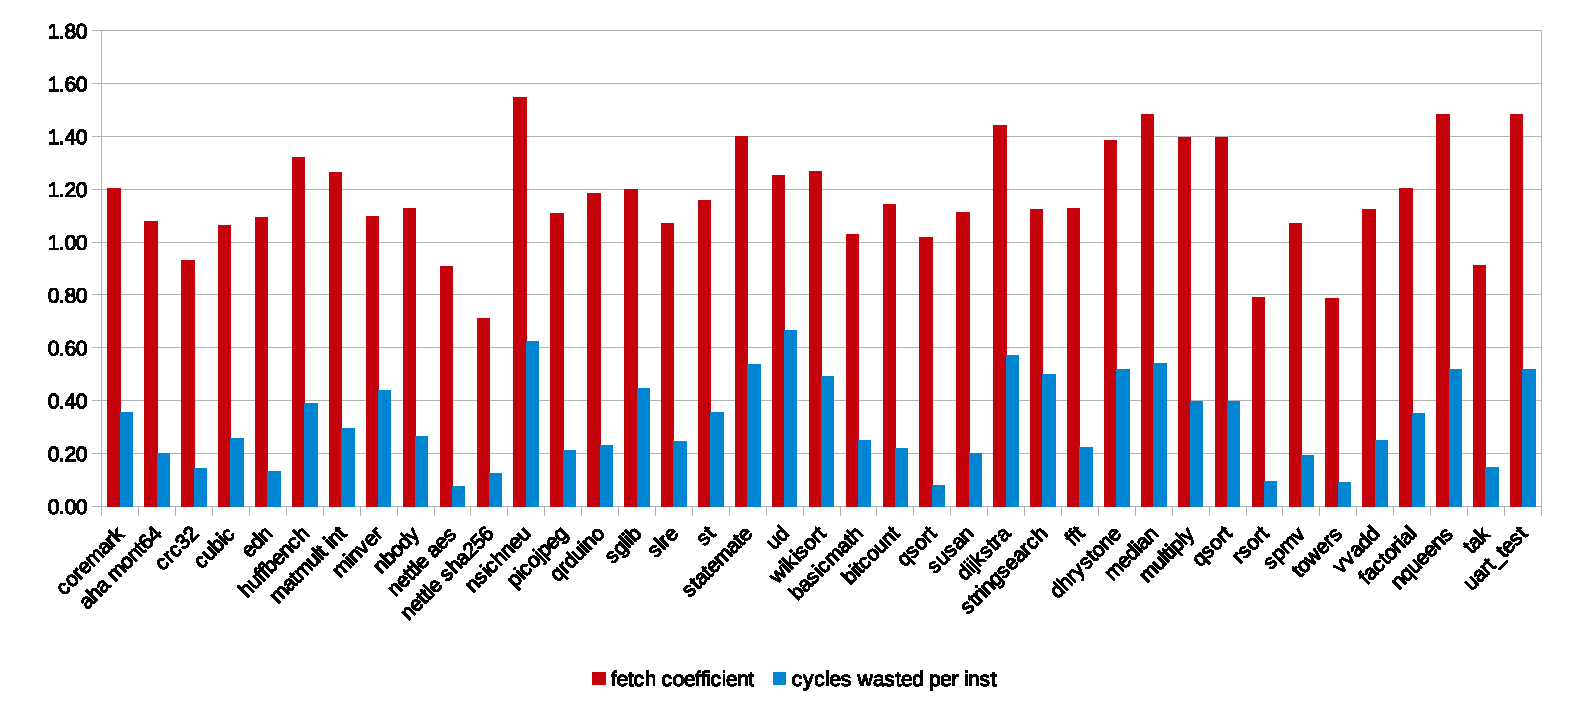
\includegraphics[width=\textwidth]{img/graph/overall_fetch_waste.eps}
    \caption{Overall load coefficient and cycles wasted per instruction of all tested benchmarking workloads}
    \label{fig:res/overall/fetch_waste}
\end{figure}

%% Dhrystone
\begin{figure}
    \centering
    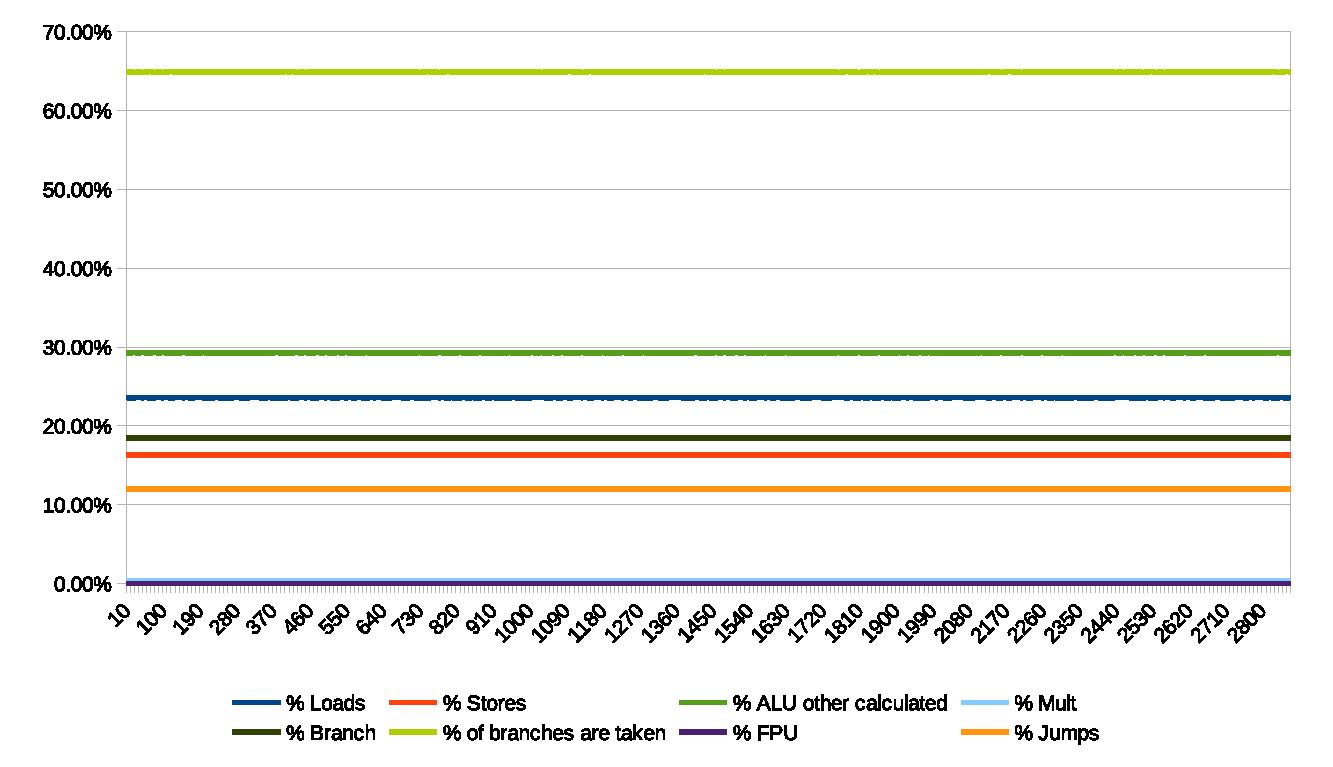
\includegraphics[width=\textwidth]{img/graph/riscv/dhrystone_inst.eps}
    \caption{Instruction distribution over time of Dhrystone (Time in ms)}
    \label{fig:res/dhrystone/inst}
\end{figure}

\begin{figure}
    \centering
    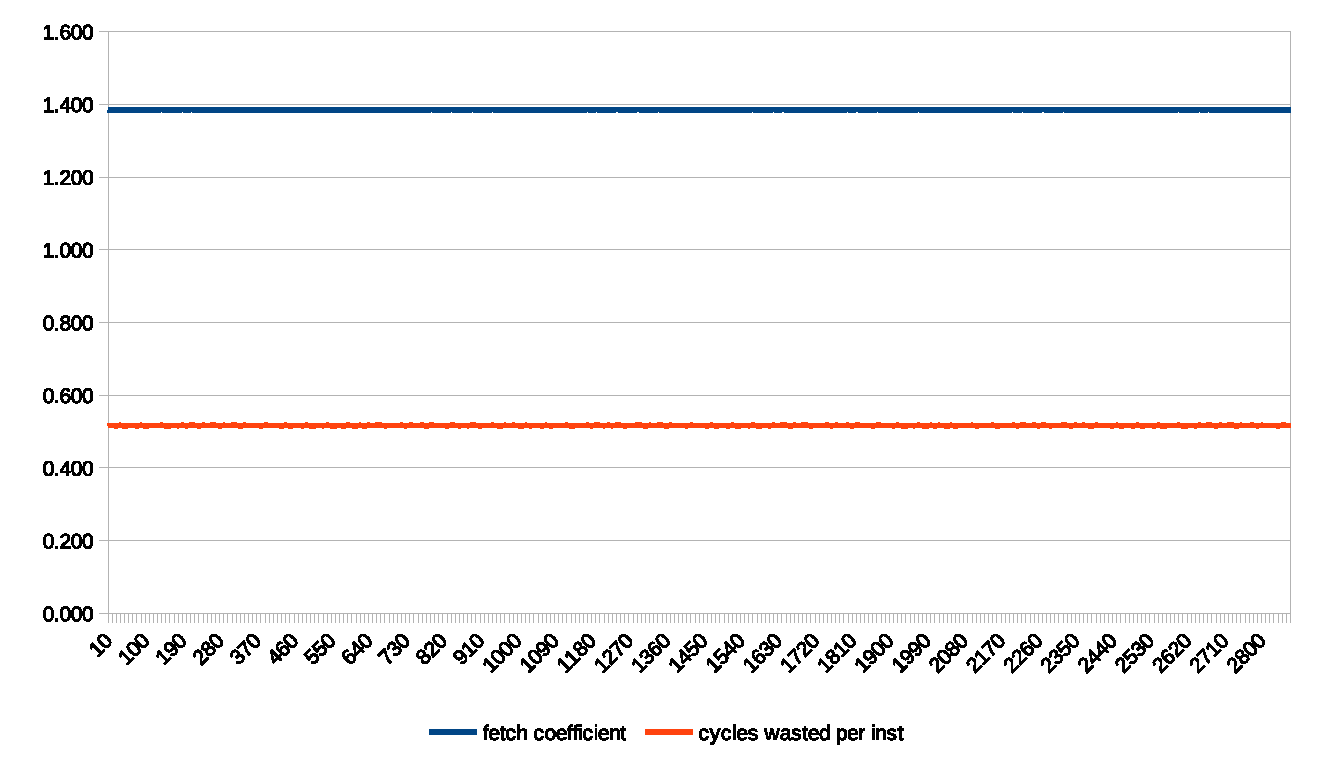
\includegraphics[width=\textwidth]{img/graph/riscv/dhrystone_fetch_waste.eps}
    \caption{Fetch coefficient and cycles wasted per instruction over time of Dhrystone (Time in ms)}
    \label{fig:res/dhrystone/fetch_waste}
\end{figure}

%% bitcount
\begin{figure}
    \centering
    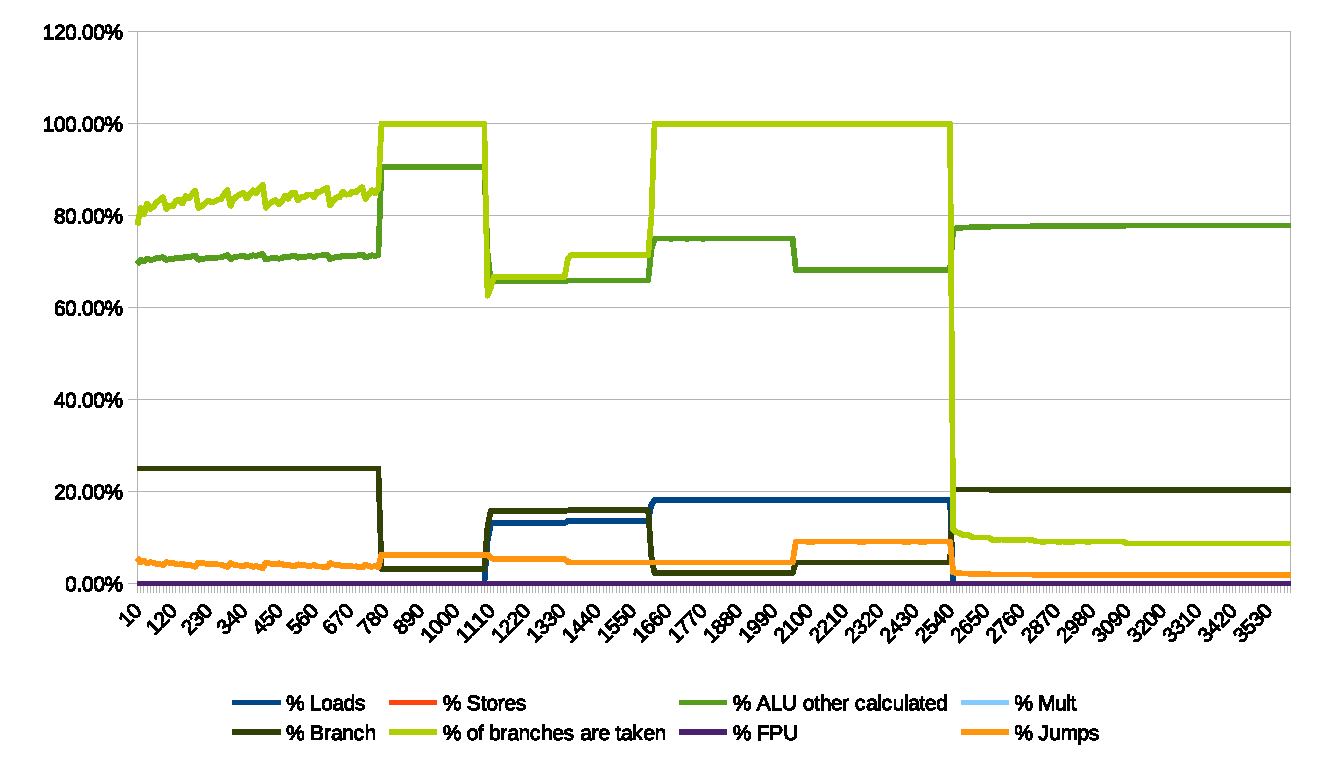
\includegraphics[width=\textwidth]{img/graph/mibench/bitcount_inst.eps}
    \caption{Instruction distribution over time of \texttt{bitcount} (Time in ms)}
    \label{fig:res/bitcount/inst}
\end{figure}

\begin{figure}
    \centering
    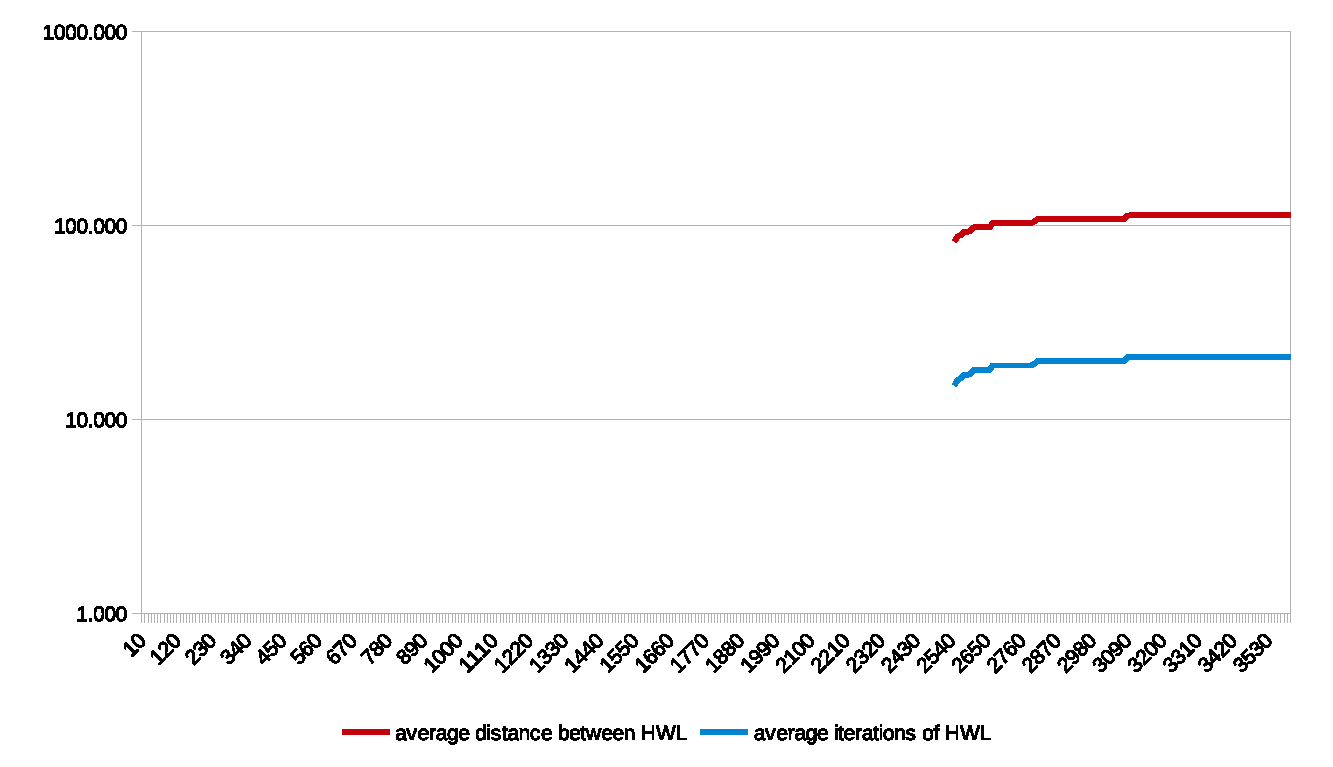
\includegraphics[width=\textwidth]{img/graph/mibench/bitcount_hwl.eps}
    \caption{Hardware loop behavior over time of \texttt{bitcount} (Time in ms)}
    \label{fig:res/bitcount/hwl}
\end{figure}

\begin{figure}
    \centering
    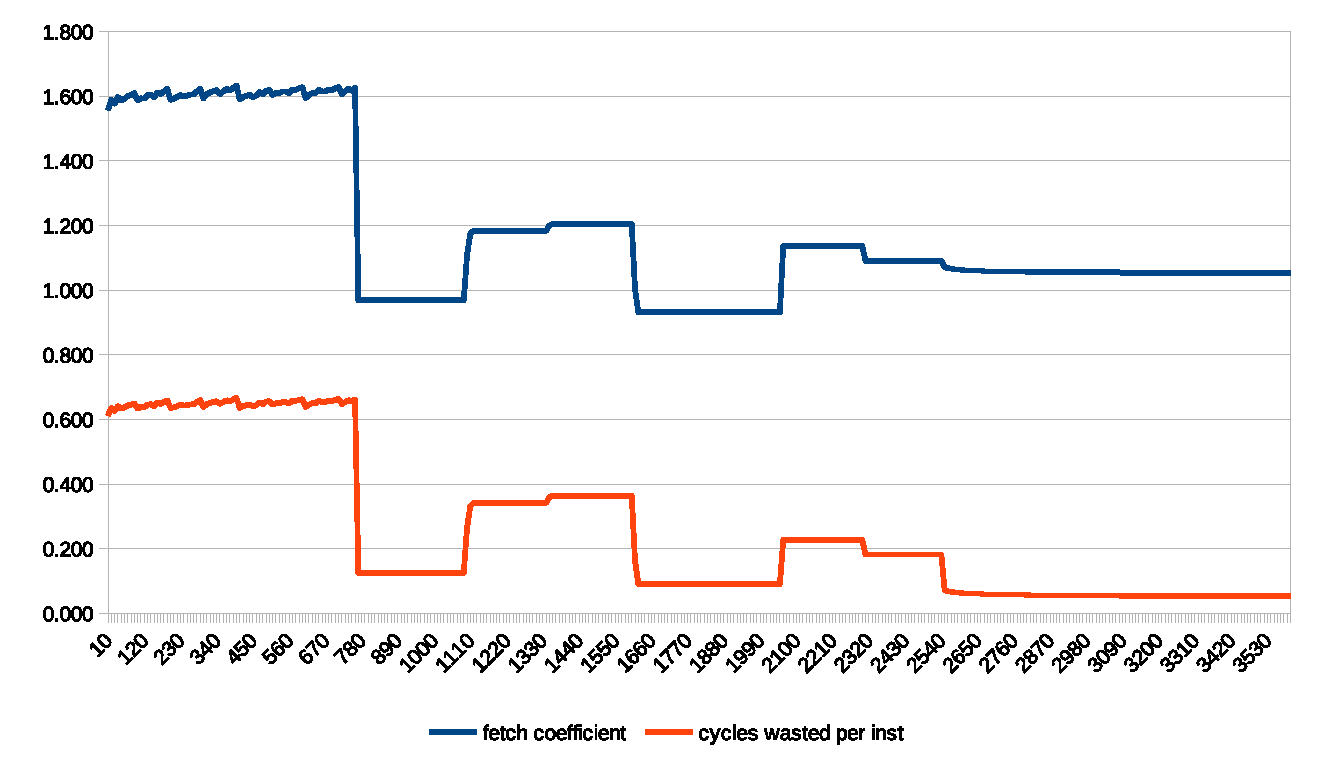
\includegraphics[width=\textwidth]{img/graph/mibench/bitcount_fetch_waste.eps}
    \caption{Fetch coefficient and cycles wasted per instruction over time of \texttt{bitcount} (Time in ms)}
    \label{fig:res/bitcount/fetch_waste}
\end{figure}

%% Coremark
\begin{figure}
    \centering
    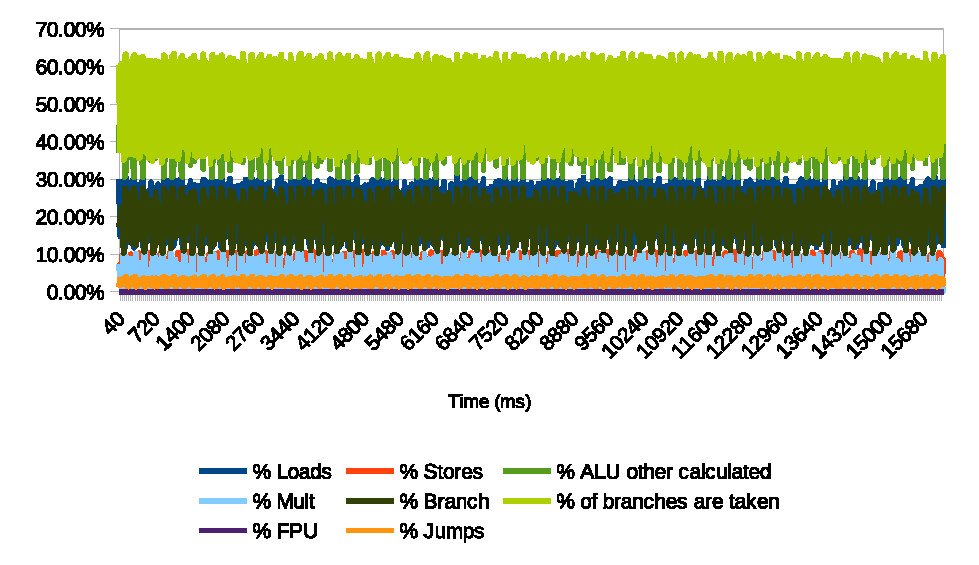
\includegraphics[width=\textwidth]{img/graph/coremark/coremark_inst.eps}
    \caption{Instruction distribution over time of Coremark (Time in ms)}
    \label{fig:res/coremark/inst}
\end{figure}

\begin{figure}
    \centering
    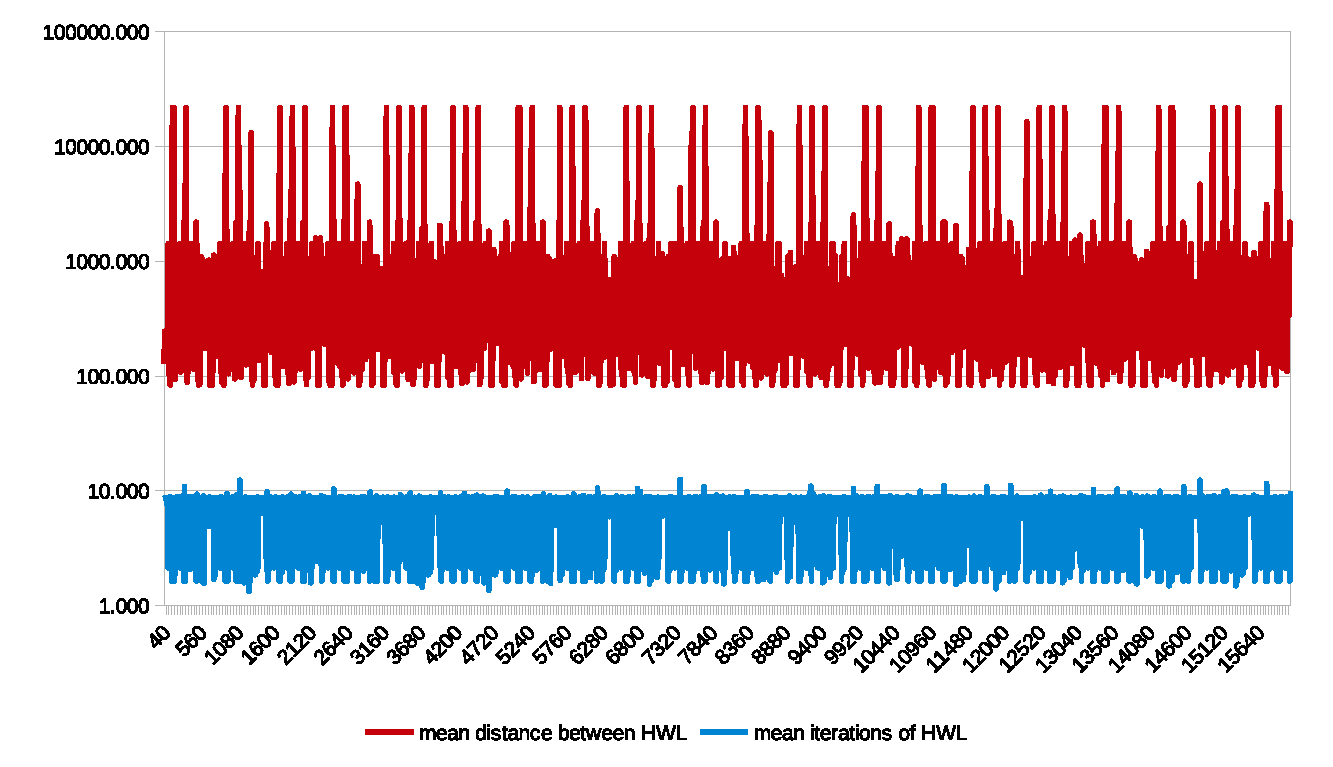
\includegraphics[width=\textwidth]{img/graph/coremark/coremark_hwl.eps}
    \caption{Hardware loop behavior over time of Coremark (Time in ms)}
    \label{fig:res/coremark/hwl}
\end{figure}

\begin{figure}
    \centering
    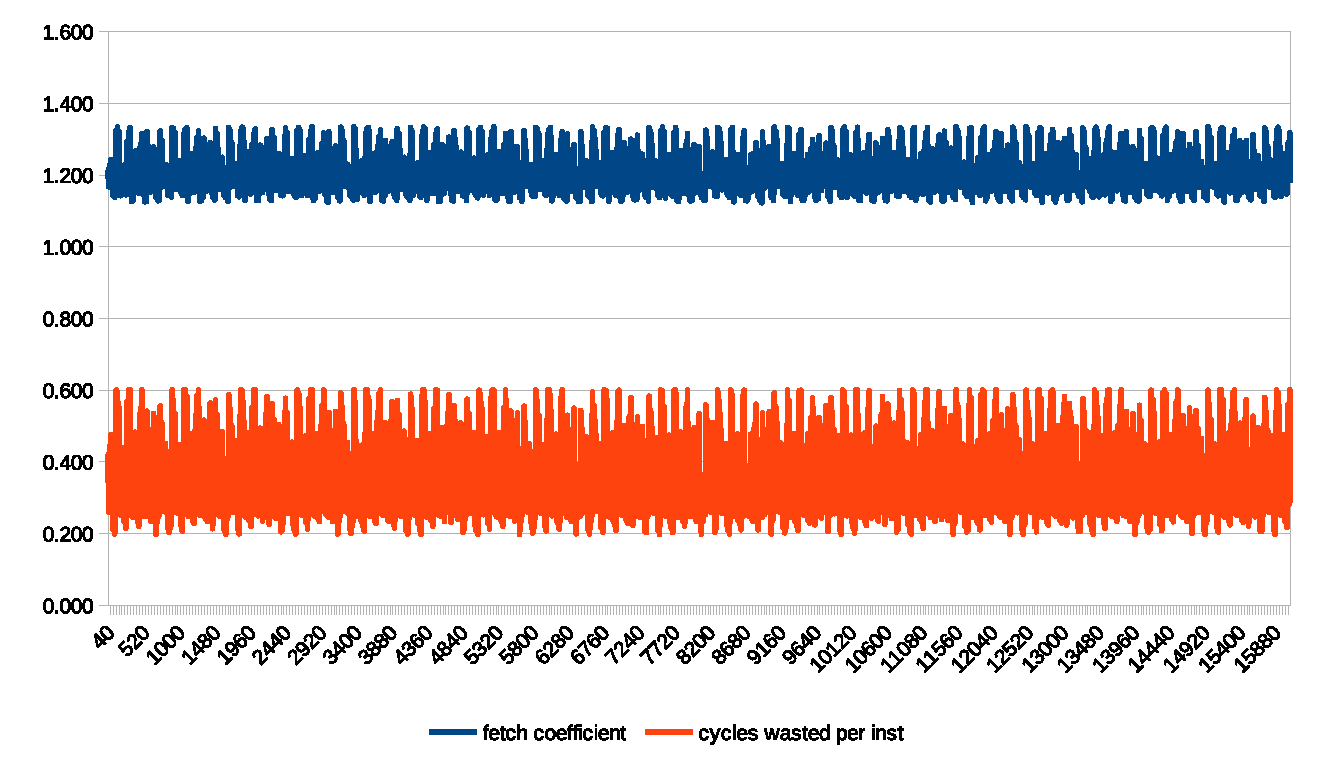
\includegraphics[width=\textwidth]{img/graph/coremark/coremark_fetch_waste.eps}
    \caption{Fetch coefficient and cycles wasted per instruction over time of Coremark (Time in ms)}
    \label{fig:res/coremark/fetch_waste}
\end{figure}

%% sglib
\begin{figure}
    \centering
    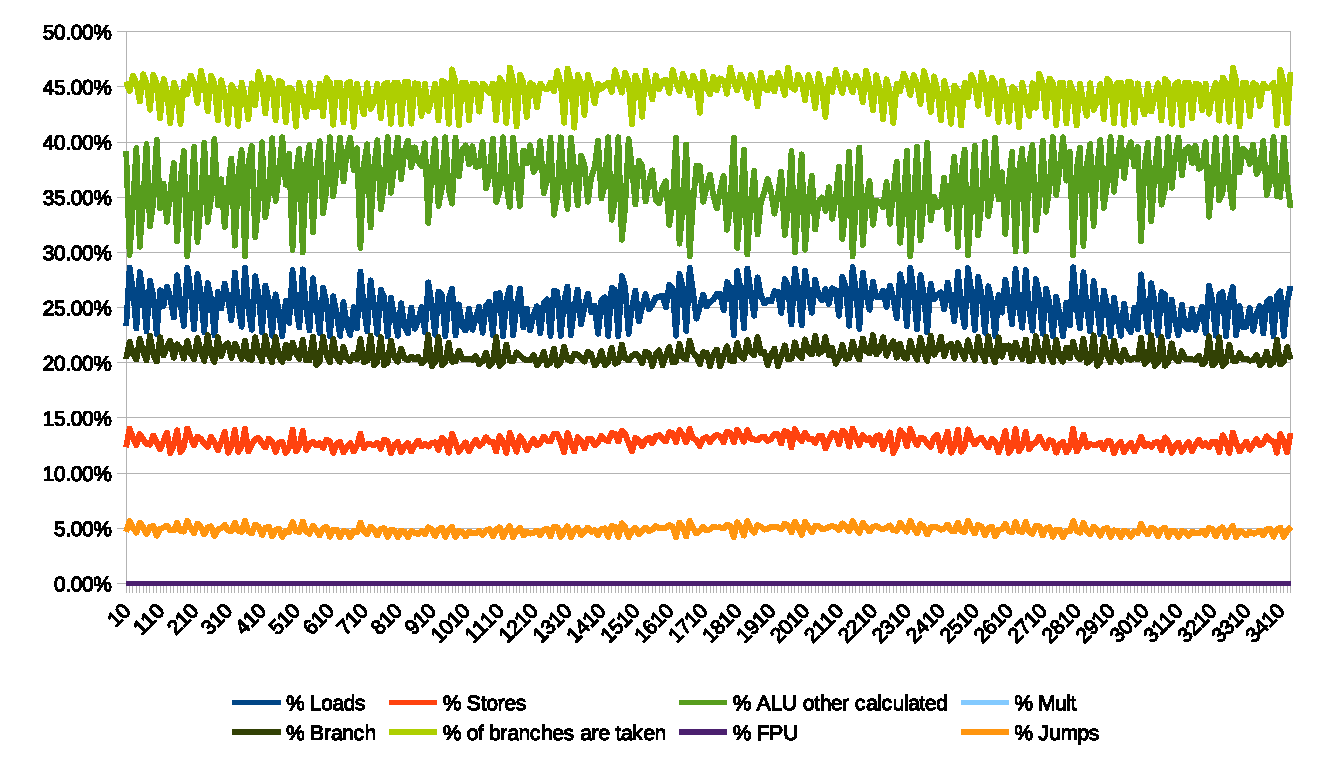
\includegraphics[width=\textwidth]{img/graph/embench/sglib-combined_inst.eps}
    \caption{Instruction distribution over time of \texttt{sglib-combined} (Time in ms)}
    \label{fig:res/sglib/inst}
\end{figure}

\begin{figure}
    \centering
    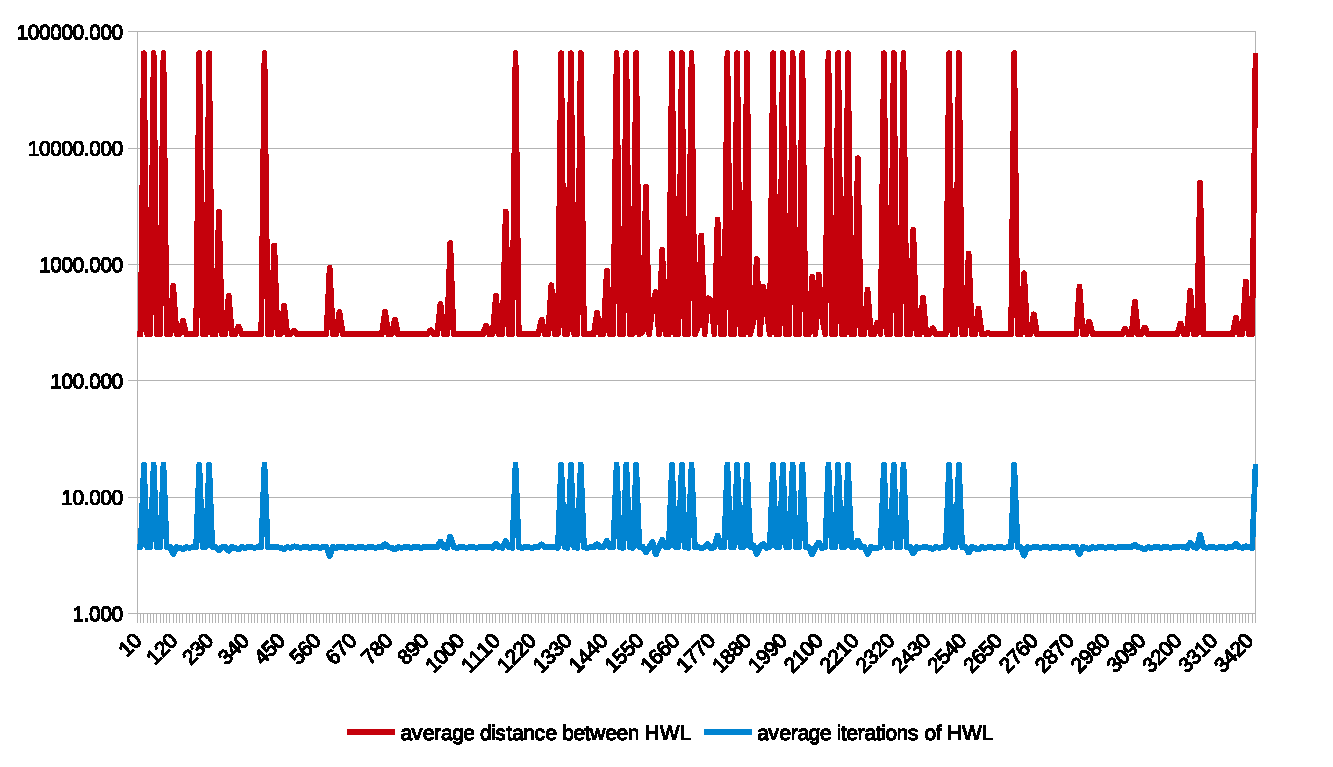
\includegraphics[width=\textwidth]{img/graph/embench/sglib-combined_hwl.eps}
    \caption{Hardware loop behavior over time of \texttt{sglib-combined} (Time in ms)}
    \label{fig:res/sglib/hwl}
\end{figure}

\begin{figure}
    \centering
    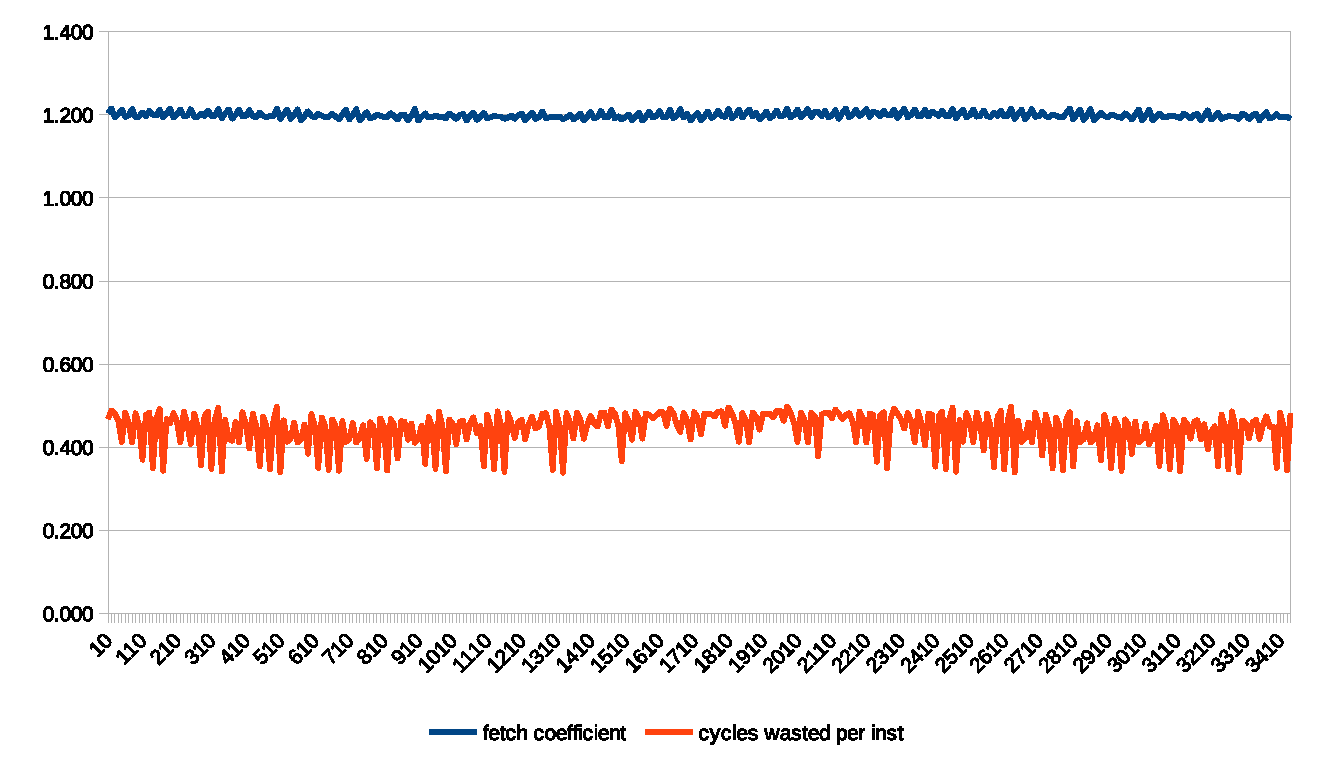
\includegraphics[width=\textwidth]{img/graph/embench/sglib-combined_fetch_waste.eps}
    \caption{Fetch coefficient and cycles wasted per instruction over time of \texttt{sglib-combined} (Time in ms)}
    \label{fig:res/sglib/fetch_waste}
\end{figure}

\section{Metric correlation}
We calculated the Pearson's correlation coefficient of the different metrics collected in order to gauge metric interdependence. As mentioned previously, a coefficient closer to 0 is desired. A metric represents a subsystem in the core and more correlation means more bias towards this subsystem in the data. Table \ref{tab:res/corr/coeff} shows the correlation coefficient between metrics. We see moderate correlation with the mean being about 0.25. We however notice a few outliers in the data. The most definite example is the correlation between the mean distance between \ac{HWL} initialization and mean \ac{HWL} iteration count. Workloads which use \acp{HWL} more often seem to strongly prefer more iterations, while workloads with more distance between \acp{HWL} favor less iterations. A possible hypothesis would be a longer loop body, however we cannot verify this with the current setup. We also see a very strong correlation between the fetch coefficient and the cycles wasted. This has to be expected as more fetches require more accesses to higher level memory systems which cause more cycles being wasted. The final strong correlation is between the fetch coefficient and the share of branching instructions. While this isn't surprising either given most workloads seem to favor \emph{branches taken}, as suppose to the implemented \emph{branches not taken}, more branching instructions directly means more instructions fetched. Surprising however is only the small correlation between the percentage of taken branches and the fetch coefficient.

\begin{table}
    \centering
    \resizebox{\textwidth}{!}{%
    \begin{tabular}{l|SSSSSSSSS}
                        & \% Branch     & {\% br. taken}    & \% FPU    & \% Jumps  & {mean dist.}  & {mean it.}    & {fetch coeff.}    & {cycles wasted /} \\
                        &               &                   &           &           & HWL           & HWL           &                   & instruction       \\
        \hline
        \% Mult         & -0.37         &  0.24             & -0.09     & -0.27     &  0.26         &  0.26         & -0.04             & -0.19             \\ \hline
        \% Branch       &               & -0.12             &  0.02     &  0.39     & -0.10         & -0.11         &  0.79             &  0.72             \\ \hline
        \% br. taken    &               &                   & -0.10     & -0.20     &  0.36         &  0.36         & -0.11             & -0.03             \\ \hline
        \% FPU          &               &                   &           & -0.01     & -0.03         & -0.03         & -0.05             &  0.13             \\ \hline
        \% Jumps        &               &                   &           &           & -0.19         & -0.18         &  0.37             &  0.45             \\ \hline
        mean dist. HWL  &               &                   &           &           &               &  1.00         & -0.19             & -0.17             \\ \hline
        mean it. HWL    &               &                   &           &           &               &               & -0.20             & -0.18             \\ \hline
        fetch coeff.    &               &                   &           &           &               &               &                   &  0.82             \\
    \end{tabular}}
    \caption{Pearson's correlation coefficient between metrics}
    \label{tab:res/corr/coeff}
\end{table}

% Render bibliograhy and acronyms if rendered standalone
\isstandalone
\bibliographystyle{IEEEtran}
\bibliography{bibliography}
\subfile{abbreviations.tex}
\fi

\end{document} 
